\chapter{Reinforcement Learning}
Author: Florian Schwarzl

\section{Principle}
The idea of reinforcement learning is one that could be compared to the way an animal, for example a dog, learns what to do and what not to. Dogs are often trained by giving them treats after they have accomplished something. On the other hand, should the dog for example chase a cat around, it is reprimanded for its behaviour. This is technically just another way of reinforcement learning. The actor, in this example a dog, is given a reward or penalty depending on the action taken. The dog learns from its interaction with the environment, it maps certain behaviour either to a reward or punishment. Learning from interaction, be it with other people or the environment, represents an integral part of our lives. Reinforcement learning describes the computational approach at this way of problem solving. Attempts to recreate this natural way of leaning have been made since the first machine learning attempts. Reinforcement learning originated from three somewhat independent sources. The first one originated around 1950 and was centred around trial and error learning, similar to what is describes above. Attempts were made to recreate this learning pattern, which originated from psychology. The second idea formed around optimisation problems and their solution. The third thread formed as an interrelation between the other two and concerns temporal-difference methods. These three methods converged into a single movement around 1980. Later on, there came a surge in popularity and machine learning in general rose to be a prominent topic. With computational capacities increasing, the options for machine learning began to increase too. Today, machine learning is more prominent than ever, with most major technology companies investing in research and new fields of application. \repeatfootcite[p. 1 ff.]{Sutton18} % ToDo: fix

\subsection{Examples of application} %Pattern Recognition
Machine learning offers a wide field of possible applications. The most prominent examples can be found in data analysis. Analysing customer behaviour and tuning services according to demand has become an industry standard. While this is a well developed field, it is less suited for reinforcement learning. In these kind of scenarios, artificial neural networks and other, similar technologies are preferred. This is partially due to the setup and time required to correctly operate a reinforcement learning environment.\repeatfootcite[p. 5 f.]{Sutton18}

\subsubsection{Pattern Recognition}
A common field of application for machine learning is pattern recognition. Pattern recognition is a broad topic consisting of subcategories such as image recognition and speech and writing identification. These fields have been developed steadily and were among the first to find widespread application. With the rise of smartphones, voice assistants like Amazon Alexa and Google Echo have become standard. These are just a few examples of possible applications. New fields like the recognition of handwriting are emerging quickly and making use of the existing knowledge and technology. Software for recognition is easily available and offers a simple entry even with normal equipment. Of all fields, pattern recognition is the one which is often used as an entry to more complicated machine learning concepts.

\subsubsection{Autonomous Driving}
A more plausible application is self-driving vehicles, the DeepRacer being one example. The reason behind this preference is often overlooked. Reinforcement learning strives in situations that require interaction, meaning that the actions of the agent change the overall situation. Another reason why  other forms of machine learning are less suited for driving is the uncertainty. How these problems are formulated will be discussed in a later section.

\section{Explanation of Terminology}
Before going into detail about the concept and theory of reinforcement learning, it is necessary to define the terms which will be used in the coming chapters. Although these terms are not formally defined this way, they will be used as described below for reasons of simplicity.
\begin{itemize}
    \item \textbf{agent / actor}: The agent represents the learning entity.
    \item \textbf{environment}: Everything relevant to the problem which the agent tries to solve. This includes the properties of the agent.
    \item \textbf{state}: A complete snapshot of the environment, capturing all aspects at a certain point in time. This is only a theoretical concept, which can only be applied in simulations, as it is not feasible to capture the environment in its entirety in a real world application.
    \item \textbf{observation}: Partial capture of the environment at a certain point in time.
    \item \textbf{action}: An activity taken by the agent. The choice is based on the current policy.
    \item \textbf{action space}: Finite set of predefined actions available to the agent.
    \item \textbf{reward}: Single value received by the agent after each step.
    \item \textbf{policy}: Defines the agents behaviour in a certain situation.
    \item \textbf{values / value function}: Estimation of the future reward which will be received by taking a certain action.
    \item \textbf{model}: Recreation of an aspect of the learning problem. A model is used most often to recreate the environment in a simulation. It can also be used to simulate the agent itself or both the environment and agent in two separate models.
\end{itemize}

\section{Comparison to other ML-concepts}
Reinforcement learning is by far not the only concept which originated for machine learning. Although trial and error based learning was one of the earliest ideas, its complexity turned out to be difficult to overcome. The defining factor for reinforcement learning is that the agent learns from interaction. This poses an entirely new area of problems and possibilities. The agent is not only affected by the environment and receives consistent stimuli, but also alters the receives stimuli with its own actions. Other forms of learning concepts rely solely on input from the environment, the agents actions do not affect future input. Machine learning concepts can be divided in different ways. The simplest form of categorisation is to divide each approach based on the way an agent receives feedback.\repeatfootcite[p. 695]{ai-modern}

\subsubsection{Reinforcement Learning}
According to this definition, reinforcement learning represents its own category. The agent gets its feedback from a series of rewards, which, based on their value, indicates if the current action is desirable or not. Figure \ref{fig:rl-concept} shows how the interaction between agent and environment takes place. The agent perceives a state \( s_t \), more precisely an observation, from the environment. Based on this observation, the agent creates the reward value \( r_t \) and decides on its next action. This action in return has an effect on the environment. Taking the DeepRacer as an example, this effect is the new position of the vehicle. The altered environment is observed again and a new observation \( s_{t+1} \) and new reward \( r_{t+1} \) are generated.

\begin{figure}
    \centering
    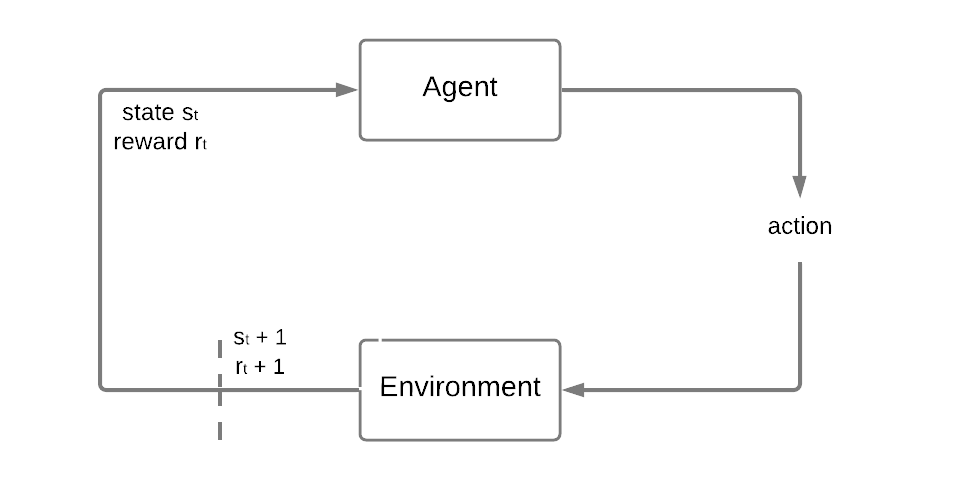
\includegraphics[width=.85\textwidth]{images/Dipl-Concept.png}
    \caption{Reinforcement learning process\repeatfootcite[p. 8]{AWS19}}
    \label{fig:rl-concept}
\end{figure}

\subsection{Supervised Learning}
The concept of supervised learning is that the learning agent has a predefined set of correctly solved examples from which it is supposed to develop a generalised hypothesis. This hypothesis is then applied to unknown examples and in the best case, solves those examples. This form of learning is used most often in image recognition, where the creation of the training set is  a manageable effort. This set is then used to create a generalised function from which the agent solves new problems. 